\documentclass[11pt]{article}
\usepackage[top=1.5cm,bottom=1.5cm,left=1cm,right=1cm]{geometry}
%\geometry{landscape}                % Activate for for rotated page geometry
\usepackage[parfill]{parskip}    % Activate to begin paragraphs with an empty line rather than an indent
\usepackage{graphicx}
\usepackage{amssymb}
\usepackage{epstopdf}
\usepackage{amsmath}            
\usepackage{multirow}    
\usepackage{hyperref}
\usepackage{changepage}
\usepackage{lscape}
\usepackage{ulem}
\usepackage{multicol}
\usepackage{dashrule}
\usepackage[usenames,dvipsnames]{color}       
\usepackage{enumerate}
\newcommand{\urlwofont}[1]{\urlstyle{same}\url{#1}}
\newcommand{\degree}{\ensuremath{^\circ}}
\newcommand{\hl}[1]{\textbf{\underline{#1}}}

\DeclareGraphicsRule{.tif}{png}{.png}{`convert #1 `dirname #1`/`basename #1 .tif`.png}

\newenvironment{choices}{
\begin{enumerate}[(a)]
}{\end{enumerate}}

% Off
\newcommand{\soln}[2]{$\:$\\ \vspace{#1}}{}
\newcommand{\solnMult}[1]{ #1 }
\newcommand{\pts}[1]{ \textbf{{\footnotesize \textcolor{black}{(#1)}}} }

%\newcommand{\soln}[2]{\textit{\textcolor{MidnightBlue}{#2}}}{}
%\newcommand{\solnMult}[1]{\textbf{\textcolor{MidnightBlue}{\textit{#1}}}}		% uncomment for solutions
%\newcommand{\pts}[1]{ \textbf{{\footnotesize \textcolor{BurntOrange}{(#1)}}} }	% uncomment for handouts

\newcommand{\note}[1]{ \textbf{\textcolor{red}{[#1]}} }	% uncomment for handouts

\begin{document}

%

Dr \c{C}etinkaya-Rundel \hfill Sta 101 \\

\begin{center}
{\LARGE Sample MT2}
\end{center}

\begin{enumerate}

\item Diamond clarity is a quality of diamonds relating to the existence and visual appearance of internal characteristics 
of a diamond called inclusions, and surface defects called blemishes. Below is a table of the currently used clarity grading 
scales for diamonds.\footnote{http://en.wikipedia.org/wiki/Diamond\_clarity} 
\begin{center}
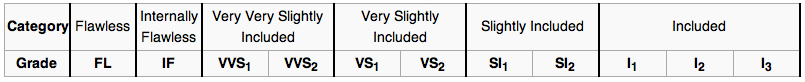
\includegraphics[width=0.8\textwidth]{figures/diamond/diamond_clarity.png} 
\end{center}
Flawless diamonds are very rare, and so are internally flawless diamonds. In a random sample of 150 diamonds, 5 
diamonds are internally flawless (IF).

\begin{enumerate}

\item What methods (theoretical, simulation, or both) can we use to construct a confidence interval for the proportion 
of diamonds that are internally flawless. Explain your reasoning.

\soln{3cm}{
We know that the sample is random and can safely assume 150 $<$ 10\% of all diamonds, so we can assume that one 
diamond in the sample is independent of another. In this sample there are 5 internally flawless diamonds (successes) 
and this is less than 10, we couldn't use theoretical methods, and must use simulation methods to construct this 
confidence interval.
}

\item Regardless of your answer to part (a), we will construct a confidence interval using a simulation -- bootstrapping. 
Explain, in your own words, how we can construct a bootstrapping distribution of 100 bootstrap statistics.

\soln{3cm}{
Sample, with replacement, 150 diamonds from the original sample and record the proportion internally flawless diamonds 
in this bootstrap sample. Repeat this 100 times and plot the distribution of the bootstrap proportions. 
}

\item Below is a bootstrap distribution of 100 bootstrap statistics. What does each dot on this distribution represent? 

\begin{minipage}[c]{0.4\textwidth}
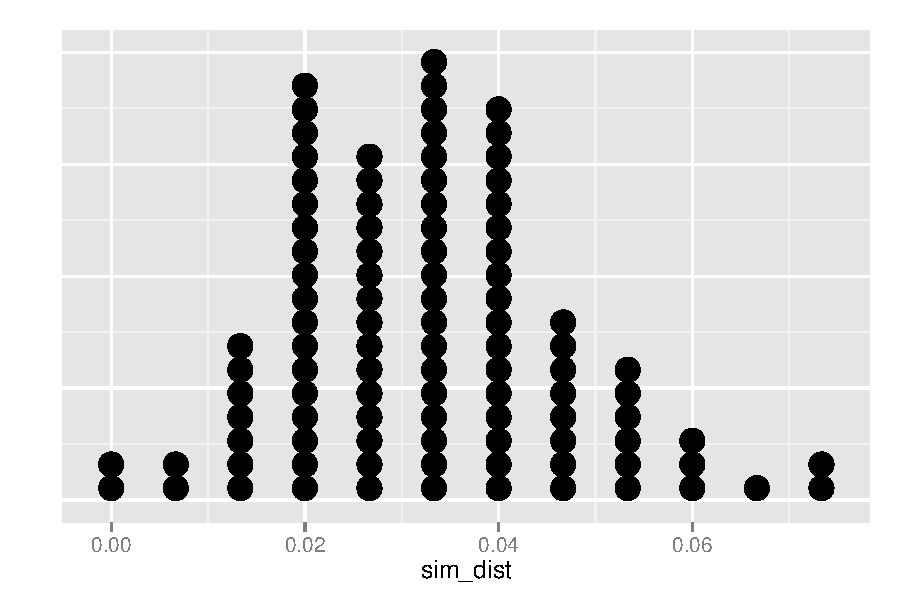
\includegraphics[width=0.9\textwidth]{figures/diamond/cl_boot_dot.pdf} 
\end{minipage}
\begin{minipage}[c]{0.05\textwidth}
\end{minipage}
\begin{minipage}[c]{0.5\textwidth}
\soln{1cm}{Each dot represents a bootstrap proportion - proportion of internally flawless diamonds in a bootstrap sample of 150 from 
the original sample.}
\end{minipage}

\vfill

%%%%%%%%%%%%%%%%%%%%%%%%%%%%%%%%%%%%%%%%%%%%%%%%%%%%%%%%%%%%%%%

\pagebreak

\item The mean of the above distribution is 0.033 and the standard deviation is 0.015. Calculate the 90\% bootstrap 
confidence interval using the percentile method as well as the standard error method.

\soln{4cm}{
\textit{Percentile method:} The bounds of the confidence interval mark the middle 90\% of the bootstrap distribution. Since 
the distribution is comprised of 100 bootstrap proportions, we find the cutoff points that mark the lower and upper 5\% 
(5 points on each end) of the distribution: (0.013, 0.06). \\
\textit{Standard error method:} $0.033 \pm 1.66 * 0.015 =  (0.00825, 0.05775)$.
}

\item Interpret the above confidence interval in context of the question.

\soln{3cm}{
We are 90\% confident that roughly 1.3\% to 6\% of all diamonds are internally flawless (based on the percentile method).
}

\end{enumerate}

%%%%%%%%%%%%%%%%%%%%%%%%%%%%%%%%%%%%%%%%%%%%%%%%%%%%%%%%%%%%%%%

\pagebreak

\item Another criterion that determines the quality of the diamond (and hence its price) is the color. Below is a table of the 
currently used clarity grading scales for diamonds.\footnote{http://www.allaboutgemstones.com/diamonds\_4cs\_color.html} 
\begin{center}
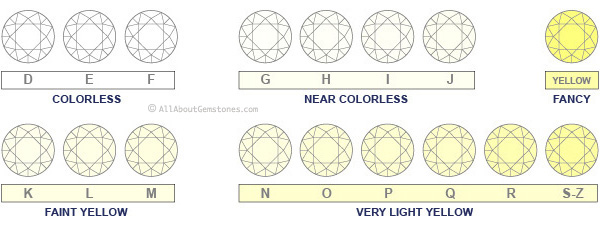
\includegraphics[width=0.6\textwidth]{figures/diamond/diamond_color} 
\end{center}
The table below shows the distribution of clarity and color in the same random sample of 150 diamonds. Clarity is divided 
into two levels: \texttt{VVS+} which represented very very slightly included or higher, and \texttt{VS-} very slightly included 
or lower.

\begin{center}
\begin{tabular}{rrr}
  \hline
 & colorless & near colorless \\ 
  \hline
VVS+ &   15 &  15 \\ 
  VS- &  64 &  56 \\ 
   \hline
\end{tabular}
\end{center}

\begin{enumerate}

\item What percent of VVS+ diamonds are colorless?

\soln{1cm}{$15 / (15 + 15) = 0.5$}

\item What percent of VS- diamonds are colorless?

\soln{1cm}{$64 / (64 + 56) = 0.533$}

\item Write the hypotheses (in words and using notation) for testing if the proportion of colorless diamonds is different 
between the VVS+ and VS- diamonds.

\soln{2cm}{$H_0: p_{VVS+} = p_{VS-}$; Proportions of colorless VVS+ and VS- diamonds are equal. \\
$H_0: p_{VVS+} \ne p_{VS-}$; Proportions of colorless VVS+ and VS- diamonds are different.}

\item What is the parameter of interest? (in words and using notation)

\soln{1cm}{Difference between the population proportions of colorless VVS+ and VS- diamonds;  $p_{VVS+} = p_{VS-}$}

\item What is the point estimate? (in words and using notation) Calculate this value.

\soln{1cm}{Difference between the sample proportions of colorless VVS+ and VS- diamonds;  \\
$\hat{p}_{VVS+} = \hat{p}_{VS-} = 0.5 - 0.533 = -0.033$}

\item Describe, in your own words, how you would conduct a randomization test using index cards.

\soln{4cm}{Start with 150 index cards, 79 that say colorless and 71 near colorless on them. Shuffle these cards and 
split them into two groups, one of size 30 for VVS+ and another of size 120 for VS-. Calculate the proportions of 
colorless diamonds (cards) in each group and find the simulated difference $(\hat{p}_{VVS+} - \hat{p}_{VS-})$. Repeat 
this may times and calculate the proportion of simulations where the difference between the two proportions is at least 
0.033, in either direction since the alternative hypothesis is two sided.}

\vfill

%%%%%%%%%%%%%%%%%%%%%%%%%%%%%%%%%%%%%%%%%%%%%%%%%%%%%%%%%%%%%%%

\pagebreak

\item Below is the histogram of a randomization distribution resulting from such randomization test using 15,000 simulations. 
Which of the following best describes the p-value? Circle one.
\begin{center}
very small $\qquad \qquad \qquad$ small $\qquad \qquad \qquad$ large $\qquad \qquad \qquad$ very large  \\
(less than 0.001) $\qquad$ (bet. 0.001 - 0.05) $\qquad$ (bet. 0.05 - 0.50)$\qquad$ (more than 0.50)
$\:$ 
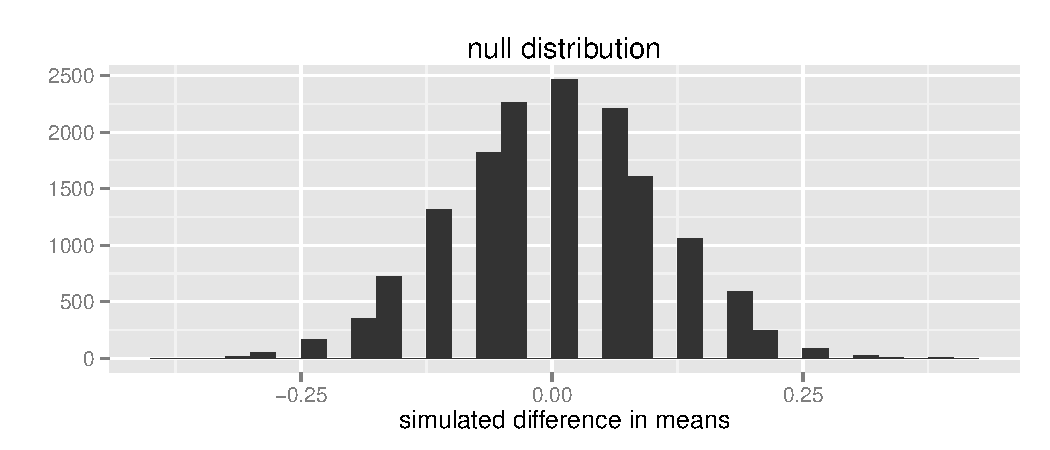
\includegraphics[width=0.7\textwidth]{figures/diamond/clar_col_ht_hist.pdf} 
\end{center}

\soln{0.001cm}{0.033 is not at all an unusual observation based on this randomization distribution, so p-value is very large}

\item What is the conclusion of the hypothesis test?

\soln{2cm}{Fail to reject the null hypothesis. The data do not provide convincing evidence that the proportion of colorless 
diamonds is different for VVS+ and VS- diamonds.}

\item Would you expect a confidence interval for the difference between the proportions of colorless VVS+ and VS- diamonds 
to include 0? Explain your reasoning. (Do not calculate a confidence interval, use the result of your hypothesis to answer this question.) 

\soln{2cm}{Since we failed to reject $H_0$ which sets the difference between the two proportions to 0, we would 
expect the confidence interval to include 0.}

\end{enumerate}


%%%%%%%%%%%%%%%%%%%%%%%%%%%%%%%%%%%%%%%%%%%%%%%%%%%%%%%%%%%%%%%

\pagebreak

\item On March 23, 2012 SurveyUSA conducted a poll in Florida on the shooting of Trayvon Martin. The table below 
shows the distribution of political ideology of respondents and the degree to which they think the victim's race was a 
factor in this shooting. \\

\begin{center}
\begin{tabular}{r c c c | c}
  \hline
 			& conservative & moderate	& liberal 	& total \\ 
  \hline
not a factor 	& 64 			&  43 		& 17 		& 124 \\ 
small factor 	& 54			&  79 		& 13 		& 146 \\ 
major factor	& 80 			& 179 		& 99		& 358 \\
not sure		& 40 			& 44 			& 26 		& 110 \\
   \hline
total			& 238		& 345		& 155 	& 738 \\
   \hline
\end{tabular}
\end{center}

\vspace{0.25cm}

\begin{enumerate}

\item What are the cases in this survey, and how many cases are there?

\soln{1cm}{Cases in this study are 738 randomly selected Florida residents.}

\item What are the variables in this study? Identify each variable as categorical or numerical.

\soln{2cm}{Variable 1: political ideology (categorical) \\
Variable 2: degree to which the respondent thinks the victim's race was a major factor in this shooting (categorical, ordinal)}

\item Name \emph{one} inference method that is appropriate for examining the relationship between the 
variables in this study? Be specific.

\soln{1cm}{Chi-squared test of independence.}

\item Write the hypotheses for testing for a relationship between these two variables. You can avoid notation 
and simply write the hypotheses in words.

\soln{3cm}{$H_0$: Political ideology and the degree to which Florida residents think the victim's race was a major factor in 
this shooting are independent of each other. \\
$H_A$: Political ideology and the degree to which Florida residents think the victim's race was a major factor in this 
shooting are associated.
}
$\:$

\item If the variables in the study are not related, how many \emph{liberal} respondents would we expect to 
have responded ``not a factor"?

\soln{2cm}{\[ E_{\text{not a factor, liberal}} = \frac{124 \times 155}{738} = 26.04 \approx 26 \]}
$\:$

\item The test statistic is calculated as 55.55. What is the p-value? Make sure to show all your work.

\soln{1cm}{$df = (R - 1) \times (C - 1) = 3 \times 2 = 6$, p-value is less than 0.001.}

\item What is the conclusion of the hypothesis test at the 5\% significance level? Interpret your conclusion 
in the context of this question.

\soln{2cm}{Reject $H_0$. The data provide convincing evidence that the political ideology and the degree to which Florida 
residents think the victim's race was a major factor in this shooting are associated.}

\end{enumerate}

%%%%%%%%%%%%%%%%%%%%%%%%%%%%%%%%%%%%%%%%%%%%%%%%%%%%%%%%%%%%%%%

\pagebreak

\item The 2010 General Social Survey asked the question; ``Do you think the use of marijuana should be made legal, 
or not?" 48\% of the 1,259 respondents said it should be made legal.

\begin{enumerate}

\item Is the number ``48\%" a sample statistic or a population parameter? Explain.

\soln{1cm}{Sample statistic, it's the observed proportion.}

\item Construct a 95\% confidence interval for the proportion of Americans who think marijuana should be made legal.

\soln{4cm}{
\begin{align*}
\hat{p} &= 0.48 \\
0.48 &\pm 1.96 \sqrt{ \frac{0.48 * (1 - 0.48)}{1259} } \\
0.48 &\pm 1.96 * 0.014 \\
0.48 &\pm 0.0274 \\
(0.4526 &, 0.5074)
\end{align*}
}
\item Interpret this confidence interval in the context of this question.

\soln{3cm}{We are 95\% confident that roughly 45.26\% to 50.74\% of Americans think marijuana should be legalized.}

\item A critic points out that this 95\% confidence interval is only accurate if the statistic follows a normal 
distribution, or if the normal model is a good approximation. Is this true for these data? Explain.

\soln{4cm}{The number of successes (people who said marijuana should be legalized: $1259 * 0.48 = 604.32$) and 
failures (people who said it shouldn't be: $1259 * 0.52 = 654.68$) are both greater than 10, therefore the distribution 
of the statistic is expected to be nearly normal.}

\item A news piece on this study's findings states; ``Majority of Americans think marijuana should be legalized." 
Based on your confidence interval, is this news piece's statement justified? 

\soln{2cm}{No, the interval contains 50\%, suggesting that the true population proportion could be just 50\% or even lower. 
Using this interval we wouldn't reject a null hypothesis where $p = 0.50$.}

\end{enumerate}

%%%%%%%%%%%%%%%%%%%%%%%%%%%%%%%%%%%%%%%%%%%%%%%%%%%%%%%%%%%%%%%

\pagebreak

\item The following histogram shows the distribution of IQ scores of fathers and mothers of a random sample of 36 
students who were identified as ``gifted" soon after they turned four. Relevant summary statistics for both 
distributions are also provided.
\footnote{Graybill, F.A. \& Iyer, H.K., (1994) Regression Analysis: Concepts and Applications, Duxbury, p. 511-6.}

\begin{minipage}[c]{0.5\textwidth}
\begin{center}
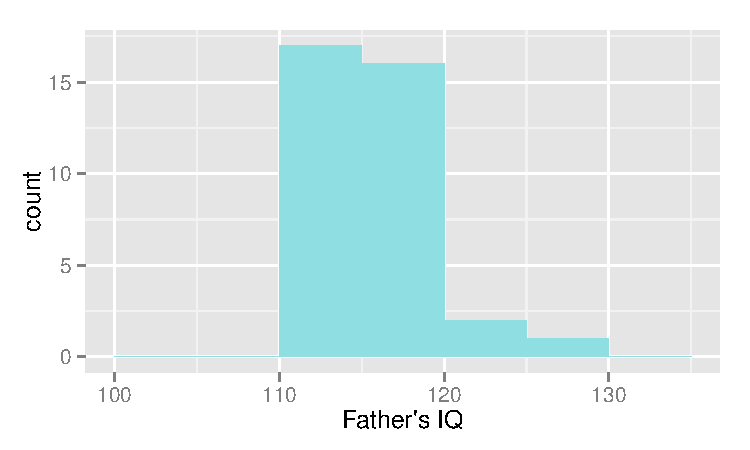
\includegraphics[width=0.8\textwidth]{figures/gifted/fatheriq_hist.pdf}
{\footnotesize
\begin{verbatim}
   Min. 1st Qu.  Median    Mean 3rd Qu.    Max. 
  110.0   112.0   115.0   114.8   116.2   126.0 
\end{verbatim}
}
\end{center}
\end{minipage}
\begin{minipage}[c]{0.5\textwidth}
\begin{center}
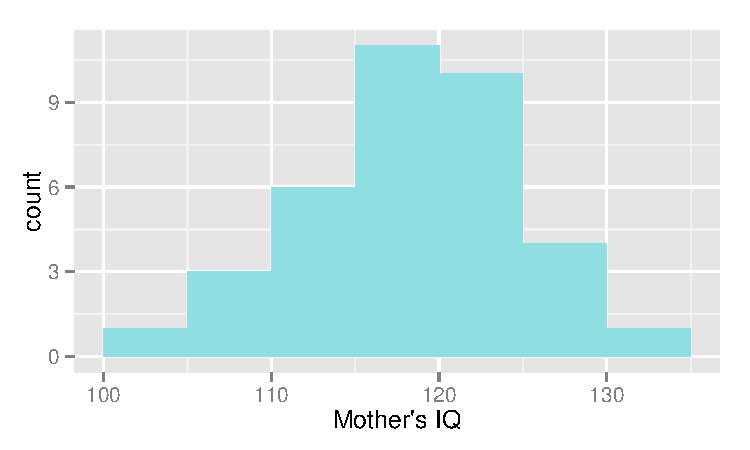
\includegraphics[width=0.8\textwidth]{figures/gifted/motheriq_hist.pdf}
\end{center}
{\footnotesize
\begin{verbatim}
   Min. 1st Qu.  Median    Mean 3rd Qu.    Max. 
  101.0   113.8   118.0   118.2   122.2   131.0 
\end{verbatim}
}
\end{minipage}

\begin{enumerate}

\item Given below is a dot plot of the bootstrap distribution of means of 15,000 bootstrap samples taken 
from the original sample of differences between the IQ scores of father and mother of a child 
(father's IQ score - mother's IQ score). 
\begin{center}
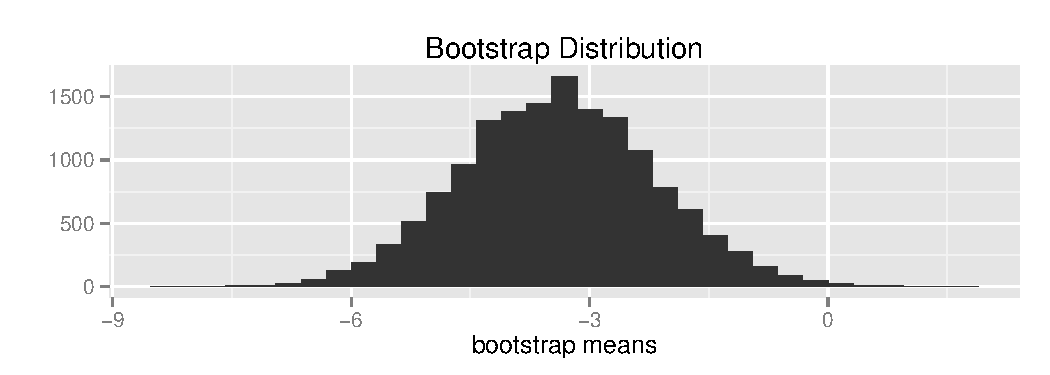
\includegraphics[width=0.9\textwidth]{figures/gifted/iqdiff_boot_hist.pdf}
\end{center}
Also provided are the cutoffs for certain percentiles of this bootstrap distribution.
\begin{verbatim}
   1%  2.5%    5%   10%   20%   80%   90%   95% 97.5%   99% 
-6.17 -5.75 -5.39 -4.94 -4.42 -2.39 -1.83 -1.36 -1.00 -0.47
\end{verbatim}
Based on this distribution, estimate a 95\% confidence interval for the true average difference between the IQ scores 
of fathers and mothers of gifted children.

\soln{1cm}{(-5.75, -1.00)}

\item Interpret this interval in context of this question. 

\vfill

\soln{2cm}{We are 95\% confident that the average IQ scores of fathers of gifted children are 5.75 points to 1 point lower than 
their mothers' IQ scores.}


%%%%%%%%%%%%%%%%%%%%%%%%%%%%%%%%%%%%%%%%%%%%%%%%%%%%%%%%%%%%%%%

\pagebreak

\item You overhear two researchers talking about this study and one of them says; ``This confidence interval 
shows that mothers of gifted children on average have significantly higher IQ scores than their fathers." Is this statement 
justified? Explain your reasoning.

\soln{2cm}{Yes, the confidence interval doesn't include 0, and both bounds are negative, suggesting mothers of gifted 
children on average have significantly higher IQ scores than their fathers.}

\item A hypothesis test for testing for the \emph{difference} between the mean IQ scores of fathers and mothers 
of gifted children yields a p-value of 0.0099. Interpret the meaning of this probability in context of this research question.

\soln{3cm}{Point estimate: $\bar{x}_F - \bar{x}_M = 114.8 - 118.2 = -3.4$\\
If in fact fathers and mothers of gifted children have on average the same IQ score, the probability of getting a sample 
of 36 gifted children where the difference between the average IQ scores of fathers and mothers is 3.4 points or more is 0.0098.}

\end{enumerate}

\vfill

%%%%%%%%%%%%%%%%%%%%%%%%%%%%%%%%%%%%%%%%%%%%%%%%%%%%%%%%%%%%%%%

\pagebreak

\begin{center}
\textit{Answer questions \ref{countF} to \ref{countL} based on the information below.}
\end{center}
$\:$
\hrule
The following histogram shows the distribution of the ages (in months) at which a random sample of 36 children first 
counted to 10 successfully. These children were identified as ``gifted" soon after they turned four.
\footnote{Graybill, F.A. \& Iyer, H.K., (1994) Regression Analysis: Concepts and Applications, Duxbury, p. 511-6.}

\begin{minipage}[c]{0.5\textwidth}
\begin{center}
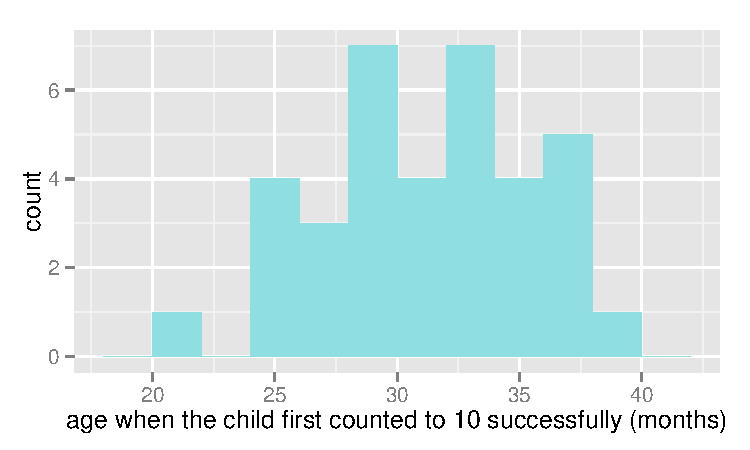
\includegraphics[width=\textwidth]{figures/gifted/count_hist.pdf}
\end{center}
\end{minipage}
\begin{minipage}[c]{0.5\textwidth}
\begin{center}
{\footnotesize
\begin{verbatim}
   Min. 1st Qu.  Median    Mean 3rd Qu.    Max. 
  21.00   28.00   31.00   30.69   34.25   39.00 
\end{verbatim}
}\end{center}
\end{minipage}
$\:$ \\
\hrule
$\:$

\item \label{countF} Which of the following is the correct set of hypotheses for testing if the average age at 
which gifted children fist count to 10 successfully is less than 32 months?

\begin{multicols}{2}
\begin{enumerate}
\item \solnMult{$H_0: \mu = 32$; $H_A: \mu < 32$}
\item $H_0: \mu = 32$; $H_A: \bar{x} < 30.69$
\item $H_0: p = 32$; $H_A: p < 32$
\item $H_0: \bar{x} = 32$; $H_A: \bar{x} < 32$
\end{enumerate}
\end{multicols}

\item Which of the following is an appropriate method for these data?

\begin{multicols}{2}
\begin{enumerate}
\item $\chi^2$ test of independence
\item $\chi^2$ test of goodness of fit
\item ANOVA
\item \solnMult{T-test}
\end{enumerate}
\end{multicols}

\item The test statistic is calculated as -1.82. Which of the below ranges contain the p-value?

\begin{multicols}{2}
\begin{enumerate}
\item Less than 0.005
\item \solnMult{Between 0.025 and 0.05}
\item Between 0.05 and 0.1
\item Greater than 0.1
\end{enumerate}
\end{multicols}

\item  \label{countL} Which of the below is the best interpretation of the p-value for this hypothesis test?

\begin{enumerate}
\item Probability that gifted children successfully count to 10 at the average age of 32 months.
\item Probability that gifted children successfully count to 10 at the average age of less than 32 months.
\item \solnMult{Probability of getting a random sample of 36 gifted children where the average age at which they 
count to 10 successfully is 30.69 or less, if in fact the true mean is 32 months}
\item Probability of getting a random sample of 36 gifted children where the average age at which they count to 10 
successfully is 30.69 or less, if in fact the true mean is less than 32 months
\end{enumerate}

\vfill

%%%%%%%%%%%%%%%%%%%%%%%%%%%%%%%%%%%%%%%%%%%%%%%%%%%%%%%%%%%%%%%

\pagebreak

\begin{center}
\textit{Answer questions \ref{relaxF} to \ref{relaxL} based on the information below.}
\end{center}
$\:$
\hrule
The 2010 General Social Survey asked the question ``After an average work day, about how many hours do you 
have to relax or pursue activities that you enjoy?" to a random sample of 1,155 Americans. A 95\% confidence 
interval for the mean number of hours spent relaxing or pursuing activities they enjoy was	
\[ (1.38, 1.92) \]
\hrule
$\:$


\item \label{relaxF} Which of the following is a valid interpretation of this interval?
\begin{enumerate}
\item 95\% of all Americans spend between 1.38 to 1.92 hrs per day relaxing or pursuing activities they enjoy.
\item If a new survey with the same sample size were to be taken, there is a 95\% chance that the mean number of 
hours spent relaxing or pursuing activities enjoyed in the sample would be between 1.38 and 1.92.
\item We are 95\% confident that, were we to repeat this survey, the mean number of hours spent relaxing or pursuing 
activities they enjoy would be between 1.38 and 1.92.
\item \solnMult{We are 95\% confident that Americans spend an average of 1.38 to 1.92 hours per day  relaxing or 
pursuing activities they enjoy.} \\
\end{enumerate}

%

\item If the researchers who conducted this survey wanted to report a confidence interval with a \emph{larger} 
margin of error based on the same sample of 1,155 Americans, what would change?
\begin{enumerate}
\item the confidence level would go down
\item \solnMult{the confidence level would go up}
\item the confidence level would stay the same \\
\end{enumerate}

%

\item \label{relaxL} If a new survey were to be done with 2,500 Americans, which of the following would be true?
\begin{enumerate}
\item \solnMult{margin of error would be smaller}
\item margin of error would be larger
\item margin of error would be about the same
\end{enumerate}

%%%%%%%%%%%%%%%%%%%%%%%%%%%%%%%%%%%%%%%%%%%%%%%%%%%%%%%%%%%%%%%

\pagebreak

\item Does Weight Watchers work? Researchers randomly divided 500 people into two equal-sized groups. One 
group spent 6 months on the Weight Watchers program. The other group received a pamphlet about controlling portion 
sizes. At the beginning of the study, the average difference in weights between the two groups was approximately 0. After 
the study, the average difference was about 8 pounds. The Weight Watchers group had the lower average weight. To 
test whether an average difference of 8 pounds could be due to chance, a statistician writes everyone's end-of-diet 
weight on an index card. He shuffles these cards together, and then deals them into two equal-sized groups. Which of 
the following best describes the expected result?

\begin{enumerate}
\item The average difference between the two stacks of cards will be about 8 pounds.
\item \solnMult{The average difference between the two stacks of cards will be about 0 pounds.}
\item If Weight Watchers was effective, the average difference between the two stacks of cards will be more than 8 pounds. \\
\end{enumerate}

%

\vspace{2cm}

\item Answer the following true / false questions. Each question is worth 1 point.
\begin{enumerate}[(a)]
\vspace{3mm} \item ( \solnMult{T} / F ) With large sample sizes even small differences between the null value and the 
point estimate, also called the effect size, can be statistically significant.
\vspace{3mm} \item ( \solnMult{T} / F ) If you found $\chi^2=10$ and df=5 you would fail to reject $H_0$ at 5\% significance level.
\vspace{3mm} \item ( T / \solnMult{F} ) A cutoff of $\alpha = 0.05$ is the ideal value for all hypothesis tests.
\vspace{3mm} \item ( \solnMult{T} / F ) We should be concerned about the independence of observations in a sample 
if we sample more than 10\% of the population without replacement.
\vspace{3mm} \item ( T / \solnMult{F} ) If the p-value is sufficiently large you can reject $H_A$.
\vspace{3mm} \item ( T / \solnMult{F} ) Power of a test and the probability of making a Type 1 error are complements.
\vspace{3mm} \item ( \solnMult{T} / F ) The equivalent confidence level for a two-sided hypothesis test with $\alpha = 0.05$ is 95\%.
\vspace{10mm}
\end{enumerate}

\end{enumerate}
%
%
\end{document}